\documentclass{classrep}
\usepackage[utf8]{inputenc}
\usepackage{color}
\usepackage{graphicx}

\DeclareUnicodeCharacter{00A0}{~}

\studycycle{Informatyka, studia dzienne, inż I st.}
\coursesemester{VI}

\coursename{Sztuczna inteligencja i systemy ekspertowe}
\courseyear{2019/2020}

\courseteacher{Krzysztof Lichy}
\coursegroup{poniedziałek, 10:15}

\author{
  \studentinfo{Paweł Białek}{216723} \and
  \studentinfo{Łukasz Kostrzewa}{216804}
}

\title{Zadanie 1: Piętnastka}

\begin{document}
\maketitle


\section{Cel}
{\color{black}
Celem zadania było napisanie programu rozwiązującego układankę zwaną "Piętnastką" za pomocą różnych metod przeszukiwania. Następnie należało dokonać porównania
skuteczności wszystkich analizowanych metod.}

\section{Wprowadzenie}
{\color{black}
Piętnastka jest to układanka zbudowana z ramki 4x4  i znajdujących się w niej 15 elementów oznacza to, że możliwe jest przesuwanie niektórych elementów ponieważ w ramce pozostaje puste miejsce.
\begin{figure}
\centering
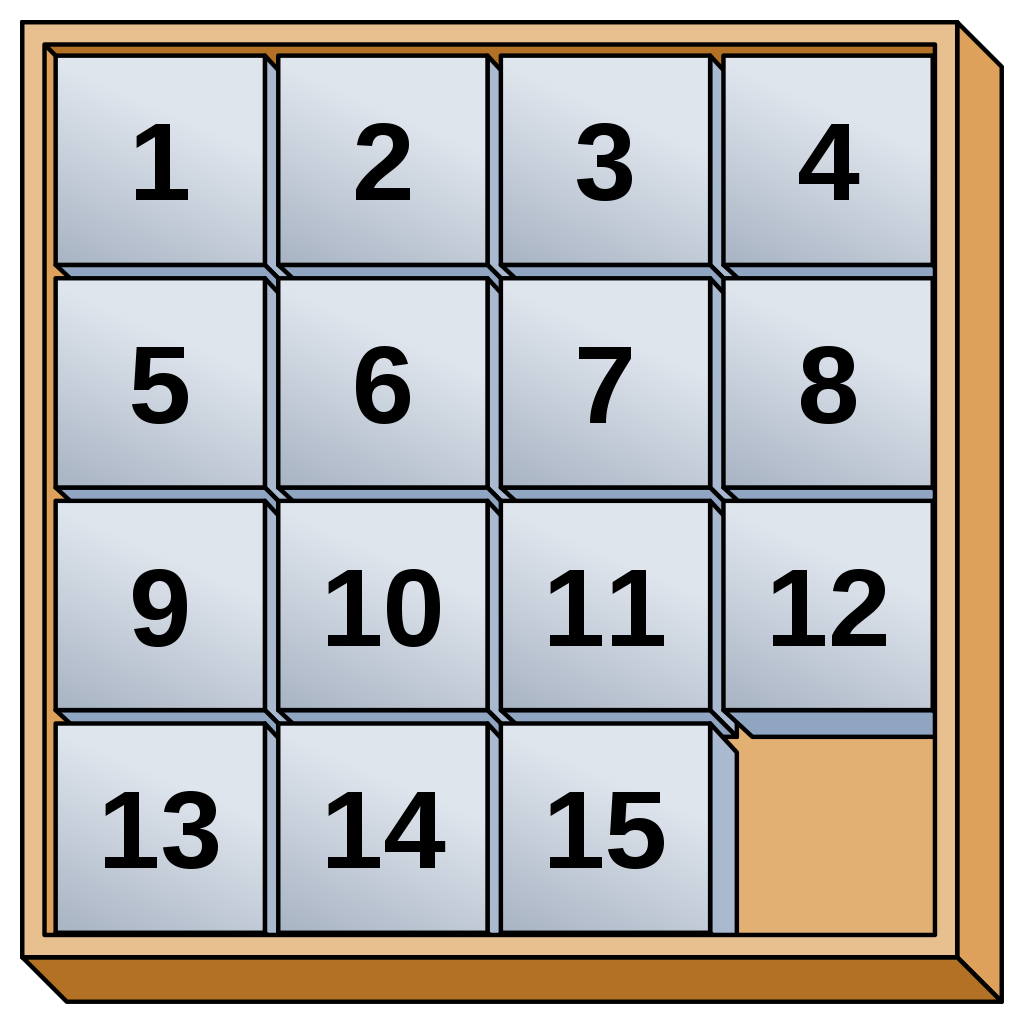
\includegraphics [scale=0.15]{1024px-15-puzzle.svg}
\caption{Rozwiązana układanka.}
\end{figure}
\newpage
W celu rozwiązania układanki użyto trzech metod przeszukiwania stanów:
\begin{enumerate}
\item Strategii przeszukiwania "wszerz" (BFS) - polega ona na przeszukiwaniu wszystkich wierzchołków na danym poziomie począwszy od stanu początkowego, po odwiedzeniu wszystkich wierzchołków przechodzi do następnego poziomu, aż do odnalezienia rozwiązania.
\item Strategii przeszukiwania "w głąb" (DFS) - polega ona na przeszukiwaniu wszystkich wierzchołków w danym korzeniu począwszy od stanu początkowego, po odwiedzeniu wszystkich wierzchołków przechodzi do następnego korzenia, aż do odnalezienia rozwiązania. 
\item Strategii "najpierw najlepszy": A*, z następującymi heurystykami: 
\begin{itemize}
\item metryką Hamminga - definicja
\item metryką Manhattan - definicja 
\end{itemize}
\end{enumerate}}

\section{Opis implementacji}
Program jest aplikacją konsolową napisaną w języku Java. Aby go uruchomić należy mieć zainstalowaną maszynę wirtualną javy oraz podać 5 parametrów podczas uruchamiania:
\begin{enumerate}
\item akronim określający wybraną strategię (bfs, dfs, astr)
\item dodatkowy parametr wybranej strategii:
\begin{itemize}
\item DFS I BFS - akronim liter R,L,U,D określający kolejność przeszukiwania (Right, Left, Up, Down)
\item A* - hamm dla heurystyki Hamminga, manh dla heurystyki Manhattan
\end{itemize}
\item nazwa pliku tekstowego z zadanym układem początkowym układanki
\item nazwa pliku tekstowego, w którym ma zostać zapisane rozwiązanie
\item nazwa pliku tekstowego, w którym mają zostać zapisane dodatkowe informacje dotyczące przeprowadzonego procesu obliczeniowego
\end{enumerate}
Na poniższym diagramie zaprezentowano strukturę aplikacji. Klasa Puzzle odpowiada za przechowywanie informacji o układzie planszy, a także pozwala na wyliczenie i wykonanie możliwych ruchów oraz porównanie przechowywanego układu do oczekiwanego układu. Klasy SolverBFS, SolverDFS i SolverAStar implementują algorytmy wykorzystywane do rozwiązywania puzzli zgodne z nazwą klasy. Klasy PuzzleLoader i PuzzleSaver odpowiadają odpowiednio za wczytanie planszy z odpowiednio skonstruowanego pliku oraz zapis do pliku wynikowego oraz pliku ze szczegółowymi informacjami o wykonaniu programu.
\newpage
\begin{figure}
\centering
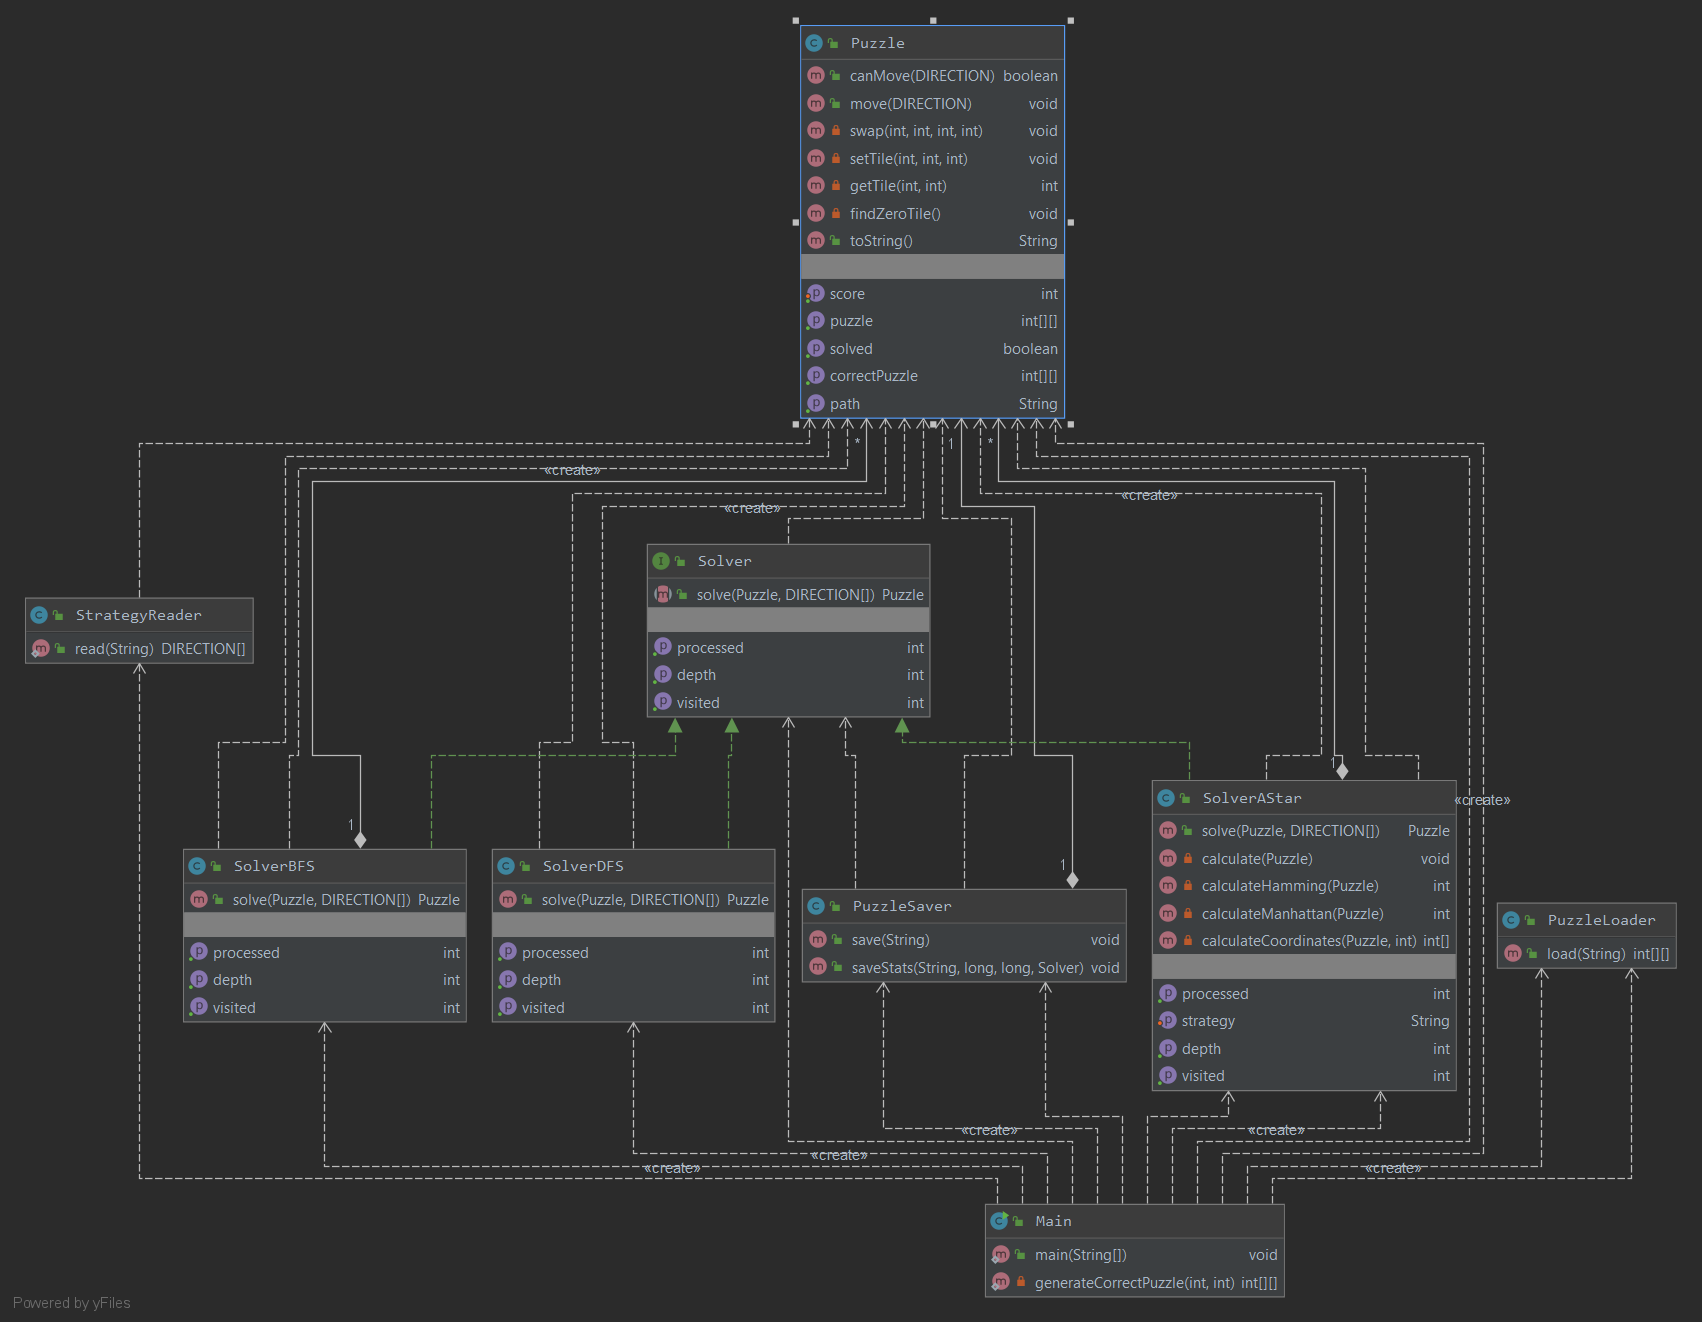
\includegraphics [scale=0.2]{SISE_Zad1_UML}
\caption{Diagram UML zawierający klasy aplikacji.}
\end{figure}


\section{Materiały i metody}
{Badania zostały przeprowadzone, na wszystkich możliwych układach do głębokości równej 7. W celu utworzenia tych układanek użyto generatora udostępnionego na platformie WIKAMP.
Następnie program uruchamiany jest dla każdej układanki i wszystkich możliwych strategii i parametrów je opisujących. Po otrzymaniu rezultatów dla wszystkich analizowanych przypadków, z utworzonych danych zostały stworzone wykresy, które zostaną przedstawionę w następnym punkcie sprawozdania. Ponieważ ilość analizowanych przypadków jest bardzo duża, w celu zebrania wszystkich danych i utworzenia odpowiednich wykresów napisano skrypt w języku python.}

\newpage
\section{Wyniki}
{
\begin{figure}[h]
\centering
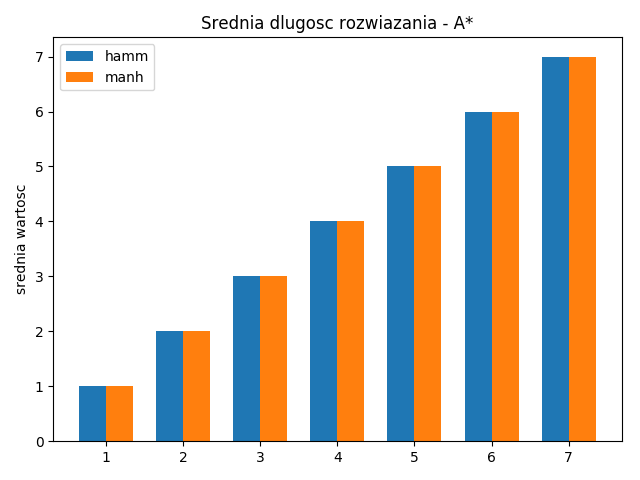
\includegraphics [scale=0.5]{dlugosc_AStar}
\caption{Wykres przedstawiający średnią długość rozwiązania dla strategii A*}
\end{figure}
\begin{figure}
\centering
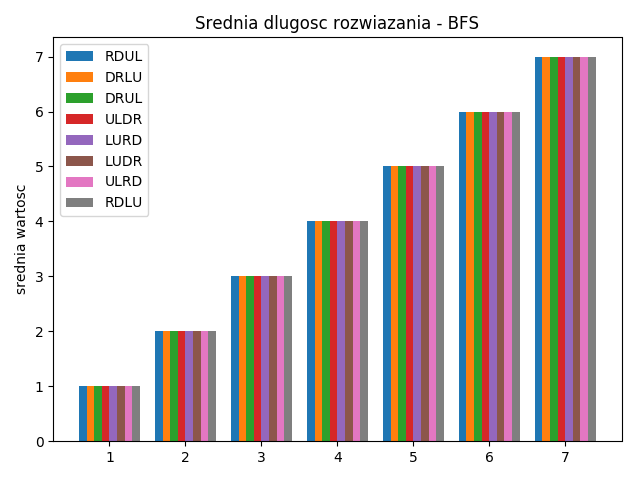
\includegraphics [scale=0.5]{dlugosc_BFS}
\caption{Wykres przedstawiający średnią długość rozwiązania dla strategii BFS}
\end{figure}
\begin{figure}
\centering
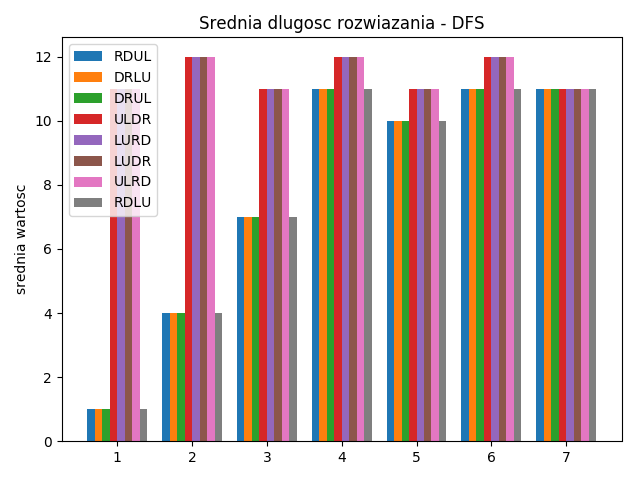
\includegraphics [scale=0.5]{dlugosc_DFS}
\caption{Wykres przedstawiający średnią ilość stanów odwiedzonych dla strategii DFS}
\end{figure}
\begin{figure}
\centering
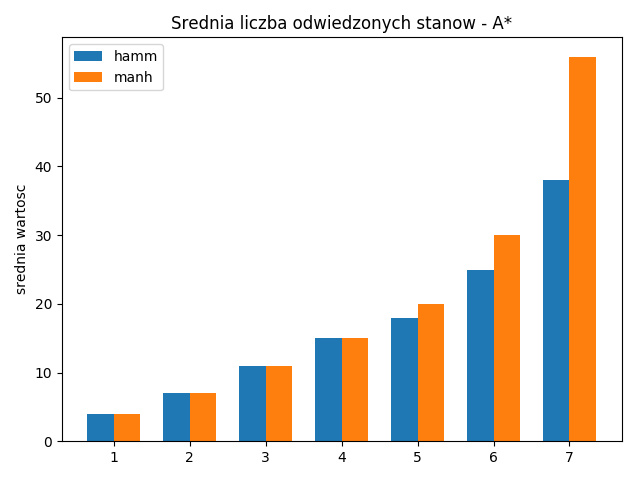
\includegraphics [scale=0.5]{odwiedzone_AStar}
\caption{Wykres przedstawiający średnią ilość stanów odwiedzonych dla strategii A*}
\end{figure}
\begin{figure}
\centering
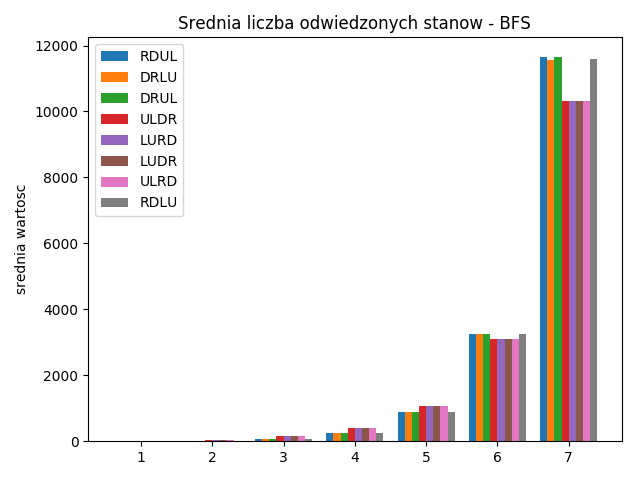
\includegraphics [scale=0.5]{odwiedzone_BFS}
\caption{Wykres przedstawiający średnią ilość stanów odwiedzonych dla strategii BFS}
\end{figure}
\begin{figure}
\centering
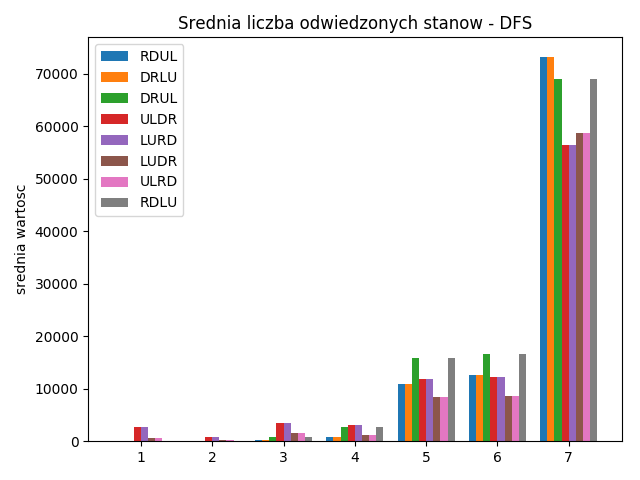
\includegraphics [scale=0.5]{odwiedzone_DFS}
\caption{Wykres przedstawiający średnią ilość stanów odwiedzonych dla strategii DFS}
\end{figure}
\begin{figure}
\centering
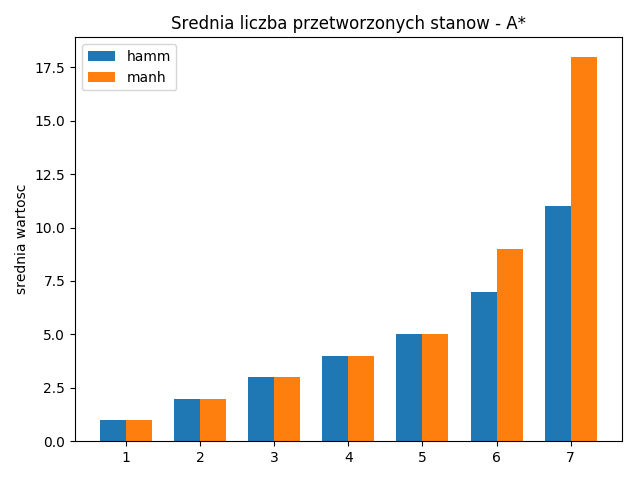
\includegraphics [scale=0.5]{przetworzone_AStar}
\caption{Wykres przedstawiający średnią ilość stanów przetworzonych dla strategii A*}
\end{figure}
\begin{figure}
\centering
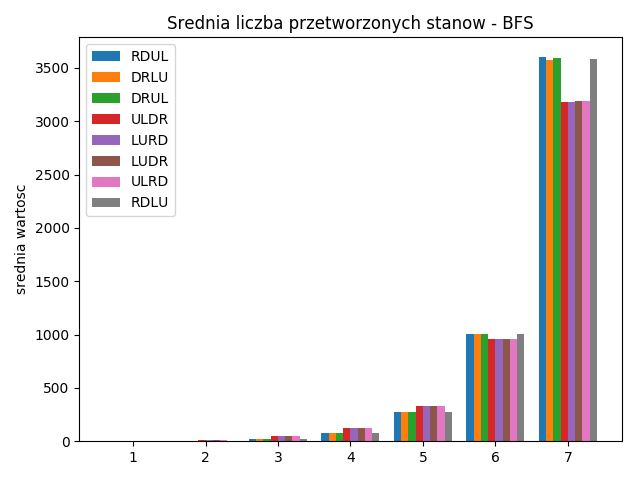
\includegraphics [scale=0.5]{przetworzone_BFS}
\caption{Wykres przedstawiający średnią ilość stanów przetworzonych dla strategii BFS}
\end{figure}
\begin{figure}
\centering
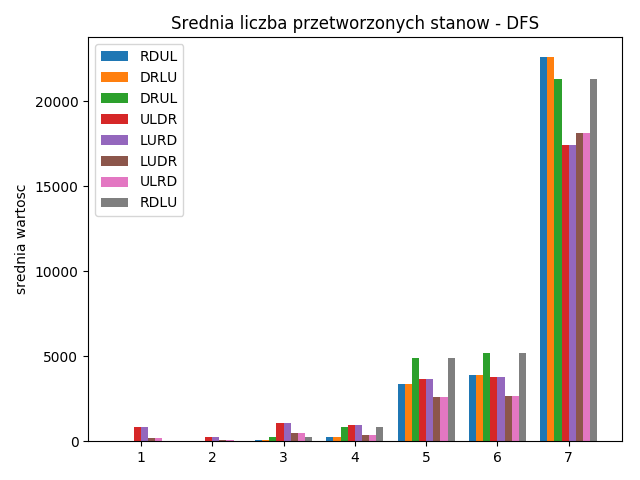
\includegraphics [scale=0.5]{przetworzone_DFS}
\caption{Wykres przedstawiający średnią ilość stanów przetworzonych dla strategii DFS}
\end{figure}
}
\newpage
\section{Dyskusja}
{\color{blue}
Sekcja ta powinna zawierać dokładną interpretację uzyskanych wyników
eksperymentów wraz ze szczegółowymi wnioskami z nich płynącymi. Najcenniejsze
są, rzecz jasna, wnioski o charakterze uniwersalnym, które mogą być istotne
przy innych, podobnych zadaniach. Należy również omówić i wyjaśnić wszystkie
napotkane problemy (jeśli takie były). Każdy wniosek powinien mieć poparcie we
wcześniej przeprowadzonych eksperymentach (odwołania do konkretnych wyników).
Jest to jedna z najważniejszych sekcji tego sprawozdania, gdyż prezentuje
poziom zrozumienia badanego problemu.}

\section{Wnioski}
{\color{blue}
W tej, przedostatniej, sekcji należy zamieścić podsumowanie najważniejszych
wniosków z sekcji poprzedniej. Najlepiej jest je po prostu wypunktować. Znów,
tak jak poprzednio, najistotniejsze są wnioski o charakterze uniwersalnym.}

\begin{thebibliography}{0}
  \bibitem{l2short} T. Oetiker, H. Partl, I. Hyna, E. Schlegl.
    \textsl{Nie za krótkie wprowadzenie do systemu \LaTeX2e}, 2007, dostępny
    online.
\end{thebibliography}

{\color{blue}
Na końcu należy obowiązkowo podać cytowaną w sprawozdaniu literaturę, z której
grupa korzystała w trakcie prac nad zadaniem.}

\end{document}
